% General Elsevier article class; numerical references remain venue-neutral.
\documentclass[preprint,12pt]{elsarticle}
\usepackage{amsmath,amssymb,booktabs,longtable,array}
\usepackage{graphicx}
\setkeys{Gin}{keepaspectratio}
\usepackage{microtype}
\setlength{\emergencystretch}{3em}
\usepackage{xcolor}
\usepackage{hyperref}
\hypersetup{colorlinks=true,linkcolor=blue,citecolor=blue,urlcolor=blue}
\newcommand{\tightlist}{\setlength{\itemsep}{0pt}\setlength{\parskip}{0pt}}
\providecommand{\pandocbounded}[1]{#1}
\makeatletter
\def\ps@pprintTitle{\let\@oddhead\@empty\let\@evenhead\@empty
  \def\@oddfoot{\footnotesize Preprint submitted to Elsevier\hfill\today}
  \let\@evenfoot\@oddfoot}
\makeatother
\begin{document}
\begin{frontmatter}
\title{When does splitting a small language model across commodity
machines pay off? Objective-aware placement, migration payback, and
recovery in Shardwise}
\author{Author names and affiliations pending}
\begin{abstract}
Pooling a few commodity machines to serve a small language model is
attractive for personal and small-group deployments, but adding a
machine does not automatically make generation faster, and
re-partitioning a running model has a cost that a short session may
never repay. We study these two decisions with Shardwise, an open,
Kubernetes-free runtime that splits a decoder-only model into contiguous
layer ranges, chooses the split with a latency (sum) or throughput
(bottleneck) objective, re-partitions on slowdown or device loss, and
admits voluntary moves only when a migration-payback test passes. We
derive the exact ordered-partition recurrence, an ideal capacity
envelope that explains when each objective is appropriate, and necessary
and sufficient payback conditions for fixed and remaining-work horizons.
In 65 completed Qwen3-0.6B runs (939 requests) on two cloud machines,
the right objective matters more than adaptation: throughput placement
serves two concurrent requests 80.5\% faster than latency placement
(7.30 vs 4.05 tokens/s), while for a single request under a 120 ms
network delay latency placement is 65.4\% faster. Adaptation to a CPU
slowdown raises fault-phase throughput by 25\%, yet only 6.8\% over the
whole run once transition and drain time are counted; measured
transitions exceed their forecast by 29-76\%; and 99.2\% of an
application-level link-cost residual is queueing rather than network
time. A remaining-work horizon suppresses moves exactly as predicted but
does not improve short sessions, because closed-loop admission renews
the work it budgets. We distil these results into deployment guidelines
and release the runtime, an installable multi-device application, and
all raw traces.
\end{abstract}
\begin{keyword}
Distributed LLM inference; Pipeline parallelism; Edge computing; Layer
partitioning; Migration cost; Reconfiguration; Performance evaluation
\end{keyword}
\end{frontmatter}
\hypertarget{introduction}{%
\section{Introduction}\label{introduction}}

Small open language models now answer everyday questions acceptably on a
laptop CPU. A student group, a small lab or a household often owns
several such machines, none of them powerful, and it is natural to ask
whether pooling them gives a faster or more robust service.
Pipeline-style distribution is the simplest way to pool them: each
machine holds a contiguous range of decoder layers and passes
activations onward \citep{huang2019gpipe, narayanan2019pipedream}.
Systems such as Petals, EdgeShard, Galaxy, TPI-LLM and prima.cpp show
that layer- or tensor-partitioned inference across edge and consumer
devices is feasible
\citep{borzunov2023petals, edgeshard2025, galaxy2024, tpi2025, prima2026}.

Feasibility, however, is not the question a deployer faces. Two
decisions determine whether pooling helps, and both are easy to get
wrong. The first is \emph{what to optimise}. Autoregressive decoding
makes one request traverse every stage for every token, so for a single
conversation each added stage adds latency; overlapping several requests
across stages is what yields speedup \citep{huang2019gpipe, yu2022orca}.
A split that maximises throughput can therefore be slower for a single
user, and the right objective depends on concurrency. The second
decision is \emph{whether to move}. When a machine slows down, leaves or
joins, the placement can be recomputed, but changing it stalls the
pipeline and, unless key-value (KV) caches are transferred, forces the
active requests to rebuild their state. Datacenter systems make such
reconfiguration cheap
\citep{sun2024llumnix, fu2024serverlessllm, miao2023spotserve}; on
commodity machines over ordinary networks it costs seconds, comparable
to the lifetime of a chat turn.

Each ingredient of these decisions has been studied. EdgeShard and later
pipeline systems distinguish latency from throughput objectives
\citep{edgeshard2025, lin2026dynopipe}; DiSCo and STAR admit a migration
only when the remaining decode work can amortise its overhead
\citep{sun-etal-2025-disco, star2026}; ServerlessLLM and Petals rebuild
inference state by replay
\citep{fu2024serverlessllm, borzunov2023petals}; and ShadowLLM and
EASTER evaluate recovery from device loss on edge hardware
\citep{chen2026shadowllmhotstandby, easter2024}. Kafetzis et al.~price
migration when re-partitioning attention heads, in simulation
\citep{kafetzis2025partitioning}, and prima.cpp re-plans only when its
task queue is empty \citep{prima2026}. What remains less understood is
how these ingredients \emph{interact} in one running service on
commodity hardware: how much of an adaptive policy's apparent gain
survives once transitions, drain and renewed work are counted, and which
measurement choices make a policy look better or worse than it is.

This paper provides that account. We build Shardwise, a compact runtime
(about 6,000 lines of Go and Python) consisting of a placement
controller, per-machine node agents, a router and layer-sharded workers,
which runs without any cluster manager. Its controller solves the
ordered contiguous partition exactly for either objective, re-partitions
on degradation or loss, and optionally gates voluntary moves by a
payback test whose horizon can be capped by the requests' remaining
output budget. We evaluate it with 65 completed real-model runs (939
requests) on two cloud machines, complemented by analytical, synthetic
and replay studies that are reported as separate evidence strata.

We ask four research questions:

\begin{itemize}
\tightlist
\item
  \textbf{RQ1} How does concurrency change the placement objective that
  serves users best?
\item
  \textbf{RQ2} When does adapting the placement repay its disruption?
\item
  \textbf{RQ3} Can a request-budget horizon make short-session move
  decisions safer?
\item
  \textbf{RQ4} Which measurement and baseline choices can reverse an
  apparent advantage?
\end{itemize}

Our main findings are:

\begin{enumerate}
\def\labelenumi{\arabic{enumi}.}
\tightlist
\item
  \textbf{Concurrency decides the objective.} With two concurrent
  requests, throughput (bottleneck) placement delivers 7.30 versus 4.05
  tokens/s for latency (sum) placement, an 80.5\% gain, and also lowers
  median completion time from 15.8 to 8.7 s. With one request under a
  120 ms delay, latency placement is 65.4\% faster (4.00 vs 2.42
  tokens/s). An ideal closed-network envelope, \(\max(B,P/Q)\), explains
  the reversal for non-speculative decoding.
\item
  \textbf{Adaptation gains shrink once costs are counted.} Adapting to a
  CPU slowdown raises fault-phase throughput by 25.0\%, but the
  whole-run gain is 6.8\%; under a network delay the adaptive policies
  are 6.4-7.6\% \emph{slower} than doing nothing. Worker loss is the
  clear case for adaptation: 19 failed requests and zero fault-phase
  output without it, none with it.
\item
  \textbf{Transition forecasts are biased low and budgets renew.}
  Measured disruptions exceed the profile-based forecast by 76.2\%
  (compute) and 29.2\% (network) on average. A remaining-work horizon
  rejects moves exactly when its payback condition predicts, yet does
  not improve short sessions, because closed-loop admission renews the
  budget it relies on.
\item
  \textbf{Telemetry and baselines can mislead.} In a controlled
  synthetic study, 99.2\% of the application-level communication
  residual is worker queueing; and improving a replica baseline's
  dispatch reverses an apparent pipeline advantage.
\end{enumerate}

Our contributions are:

\begin{itemize}
\tightlist
\item
  \textbf{C1} A precise decision model for contiguous-layer placement
  with an exact \(O(WL^2)\) recurrence for both objectives, an ideal
  capacity envelope that links them through concurrency, and necessary
  and sufficient payback conditions for fixed and remaining-work
  horizons, with sensitivity to forecast error (Section 4).
\item
  \textbf{C2} Shardwise, an open runtime and installable application
  that splits a model across any number of machines without a cluster
  manager, recovers from device loss, and lets machines join without
  accepting inbound connections (Section 3, Section 7). These are
  engineering properties, not claims of priority; firewall traversal,
  for example, is also supported by Petals through relays
  \citep{petalsacl2023}.
\item
  \textbf{C3} An audited run-level evaluation that quantifies when
  objective choice and adaptation help, retains every failure, and
  separates phase metrics from whole-run outcomes (Section 6).
\item
  \textbf{C4} Diagnostic studies of transition forecasting, telemetry
  contamination, cost-term omission and baseline design, distilled into
  practical guidelines (Sections 6.4 and 8).
\end{itemize}

The underlying principles (sum/max chain partitioning, amortised
migration, replay-based state reconstruction, Little's law) are
established
\citep{bokhari1988partitioning, pinar2004partitioning, star2026, fu2024serverlessllm, little1961proof}.
Our contribution is their combination in one small, inspectable system
with explicit replay accounting, and a careful measurement of how they
behave, and fail, in practice.

Section 2 reviews related work. Section 3 describes Shardwise and
Section 4 its decision model. Section 5 presents the methodology and
Section 6 the results. Section 7 validates multi-device deployment and
correctness. Section 8 discusses guidelines and threats to validity, and
Section 9 concludes.

\hypertarget{background-and-related-work}{%
\section{Background and related
work}\label{background-and-related-work}}

\hypertarget{pipeline-inference-and-placement}{%
\subsection{Pipeline inference and
placement}\label{pipeline-inference-and-placement}}

In pipeline parallelism a model is cut into consecutive stages placed on
different devices \citep{huang2019gpipe, narayanan2019pipedream}. For
inference, a single autoregressive request occupies one stage at a time,
so stage utilisation comes from overlapping independent requests, as in
continuous or iteration-level batching \citep{yu2022orca, kwon2023vllm}.
Pipelined speculative decoding can also fill idle stages for a single
request \citep{pipeinfer2024, flowspec2025}; Shardwise does not
speculate, so our single-request results apply to plain autoregressive
decoding. Assigning consecutive layers to an ordered set of processors
to minimise the bottleneck is the classical chains-on-chains
partitioning problem, solvable exactly by dynamic programming and faster
specialised algorithms
\citep{bokhari1988partitioning, pinar2004partitioning}; minimising the
sum is the corresponding sequential problem. Device-placement for DNN
inference across edge and cloud was established by Neurosurgeon and
related work \citep{kang2017neurosurgeon, li2020edgeai}. Shardwise uses
an exact dynamic program for both objectives with heterogeneous speeds,
context-dependent layer costs, endpoint (embedding and head) costs and
per-hop link costs; its algorithmic novelty is not claimed.

\hypertarget{distributed-llm-inference-on-edge-and-consumer-devices}{%
\subsection{Distributed LLM inference on edge and consumer
devices}\label{distributed-llm-inference-on-edge-and-consumer-devices}}

EdgeShard formulates joint device selection and partitioning for latency
and, separately, for throughput, and evaluates both on edge testbeds
\citep{edgeshard2025}. Galaxy combines tensor and sequence parallelism
with communication overlap for collaborative edge inference
\citep{galaxy2024}. TPI-LLM uses tensor parallelism and memory
scheduling to run larger models on low-resource devices \citep{tpi2025}.
MDI-LLM pipelines recurrently with per-sequence KV caches on Jetson
boards \citep{mdi2025}. prima.cpp runs large models on heterogeneous
home devices over Wi-Fi with piped-ring parallelism \citep{prima2026}.
Petals serves models cooperatively over the internet with fault
tolerance \citep{borzunov2023petals}, and Parallax addresses
decentralised allocation and routing \citep{tong2025parallax}. EdgeATP
adapts tensor parallelism across edge clusters \citep{wang2026edgeatp},
and DynoPipe moves pipeline boundaries dynamically between edge and
cloud \citep{lin2026dynopipe}. These systems deliver stronger capacity
aggregation than Shardwise, typically for models that do not fit one
device. Our study is complementary: for a model that \emph{does} fit one
machine, we ask when distribution and adaptation help a running service
at all.

\hypertarget{runtime-reconfiguration-and-migration}{%
\subsection{Runtime reconfiguration and
migration}\label{runtime-reconfiguration-and-migration}}

Kafetzis et al.~re-partition attention heads online with an explicit
migration term that includes KV-cache size, evaluated in simulation
\citep{kafetzis2025partitioning}. ATSInfer adapts tensor placement on
consumer CPU/GPU systems and suppresses rescheduling with a deviation
threshold and a minimum interval \citep{liu2026atsinfer}. Llumnix
migrates live requests among serving instances \citep{sun2024llumnix},
ServerlessLLM reduces startup and migration latency
\citep{fu2024serverlessllm}, and SpotServe re-parallelises under
preemption \citep{miao2023spotserve}. Disaggregated serving separates
prefill and decode across machines
\citep{patel2024splitwise, zhong2024distserve}. In datacenters, live
pipeline reconfiguration completes in milliseconds
\citep{bai2026pipelive, yuan2026remp}; on commodity CPUs over ordinary
networks we measure seconds. Cost-aware admission of moves is
established: DiSCo migrates a stream between device and server only when
the remaining decode savings exceed the handover overhead
\citep{sun-etal-2025-disco}, and STAR filters decode-phase migrations
that cannot amortise their cost over the remaining output
\citep{star2026}. State reconstruction is also established:
ServerlessLLM moves token history and recomputes the KV cache
\citep{fu2024serverlessllm}, Petals replays activations to rebuild a
lost stage \citep{borzunov2023petals}, and CacheGen chooses between
compressed KV transfer and recomputation by bandwidth
\citep{cachegen2024}. Shardwise replays the whole token history through
a re-partitioned chain of contiguous layers. Our question is not whether
such gates or replays can be built, but how much they matter in a
running service when the remaining work is short, transitions are
underpriced and new requests keep arriving.

On edge hardware, ShadowLLM keeps hot standbys to accelerate recovery on
Jetson boards and smartphones \citep{chen2026shadowllmhotstandby}, and
EASTER learns transformer splits that keep working, approximately, when
devices drop out \citep{easter2024}. Shardwise's recovery is exact but
slower: it re-places all layers on the survivors and replays.

\hypertarget{measurement-methodology}{%
\subsection{Measurement methodology}\label{measurement-methodology}}

Sound performance claims require reporting variability, retaining
failures and matching baselines
\citep{jain1991art, hoefler2015benchmarking}. That end-to-end timings
mix queueing and remote computation into apparent network time is a
known pitfall; a recent study of pipeline shards on AI PC fleets
corrects its own ``network time'' for exactly this reason
\citep{aipcfleet2026}. We quantify how large the contamination can be
(Section 6.4). We follow these principles: runs are the analysis unit,
all failures remain in denominators, and phase-level and whole-run
metrics are reported side by side.

Table 1 contrasts scope and evidence. Published throughput figures use
different models, hardware and batching protocols; they provide context,
not a cross-system ranking.

\begin{table}[p]
\centering\scriptsize\setlength{\tabcolsep}{4pt}
\caption{Scope and evidence of related systems. Statements summarise the cited publications; without a matched experiment, no cross-system performance ranking is implied.}
\begin{tabular}{>{\raggedright\arraybackslash}p{.19\linewidth}>{\raggedright\arraybackslash}p{.35\linewidth}>{\raggedright\arraybackslash}p{.35\linewidth}}
\toprule System & Principal capability & Relation to this study\\\midrule
EdgeShard \cite{edgeshard2025} & Separate latency/throughput optimization, device and memory constraints & Broader placement space and larger models; we examine short-run transition effects.\\
Kafetzis et al. \cite{kafetzis2025partitioning} & Migration-aware attention-head optimization; simulator evaluation & Finer allocation and explicit resources; our complementary evidence executes a full model on two VMs.\\
TPI-LLM \cite{tpi2025} & Tensor parallelism and memory scheduling on constrained devices & Stronger large-model and consumer-device evidence; different parallelization and state movement.\\
MDI-LLM \cite{mdi2025} & Recurrent pipeline, per-sequence KV caches, Jetson tests & Demonstrates capacity beyond one device; our study focuses on objective changes and transition accounting.\\
Galaxy \cite{galaxy2024} & Heterogeneity-aware hybrid parallelism and communication overlap & Richer parallelization than our serialized stage model.\\
Petals / Parallax \cite{borzunov2023petals,tong2025parallax} & Distributed block serving / decentralized allocation and routing & Broader distributed deployment than our fixed worker order.\\
Llumnix / ServerlessLLM \cite{sun2024llumnix,fu2024serverlessllm} & Stateful request migration / startup and migration-aware serving & Stronger serving and state-management mechanisms; our transition uses history replay.\\
DiSCo / STAR \cite{sun-etal-2025-disco,star2026} & Migration admitted only if remaining decode savings amortise its cost & Same payback principle for request migration; we study it for contiguous-layer re-partitioning with whole-chain replay.\\
ShadowLLM / EASTER \cite{chen2026shadowllmhotstandby,easter2024} & Hot-standby recovery / split robustness on edge boards & Physical edge recovery evidence; our recovery is exact (replay) but measured on VMs and containers.\\
SpotServe \cite{miao2023spotserve} & Adaptive parallel configurations on preemptible resources & Broader resource-reconfiguration problem than a two-worker loss test.\\
ATSInfer / ETCInfer \cite{liu2026atsinfer,lu2026etcinfer} & Consumer CPU/GPU scheduling / thermal and cooling control & Different resource and physical-control scope; quota injection is not thermal evidence.\\
prima.cpp \cite{prima2026} & Piped-ring parallelism for large models on heterogeneous home devices over Wi-Fi & Real home-device evidence and capacity aggregation; re-plans only when idle, whereas we study mid-session moves.\\
Shardwise (this work) & Exact sum/bottleneck contiguous placement, payback-gated re-partitioning, recovery, outbound-only joining & Audited real-model runs with transition, telemetry, cost-term and baseline diagnostics; capacity aggregation and prior-system comparison remain future work.\\
\bottomrule
\end{tabular}
\end{table}


\hypertarget{shardwise-design}{%
\section{Shardwise design}\label{shardwise-design}}

\hypertarget{goals}{%
\subsection{Goals}\label{goals}}

Shardwise targets a small group of trusted machines on one local
network. Its goals are: (G1) run real model inference split across any
number of machines; (G2) choose a split appropriate to the workload;
(G3) keep serving when a machine slows down or disappears; (G4) avoid
moves that cost more than they return; and (G5) require no cluster
manager, root privileges on joining machines, or inbound firewall
changes on them.

\hypertarget{architecture-and-data-path}{%
\subsection{Architecture and data
path}\label{architecture-and-data-path}}

Figure 1 shows the runtime. A router receives token-ID requests and
drives generation. Workers each hold a contiguous range of decoder
layers; the first stage embeds tokens and the last applies the final
normalisation and output head. For every token step the router issues a
remote procedure call to each active stage in order, and activations
return to the router between stages. Workers keep per-request KV caches
for their own layers. The controller computes layouts and pushes them
with a monotonically increasing \emph{generation} number;
reconfiguration is serialised against compute, so a forward pass never
runs on partially replaced weights. When the generation changes
mid-request, the router replays the request's token history through the
new chain to rebuild KV state and then continues decoding. No KV cache
is transferred.

\begin{figure}
\centering
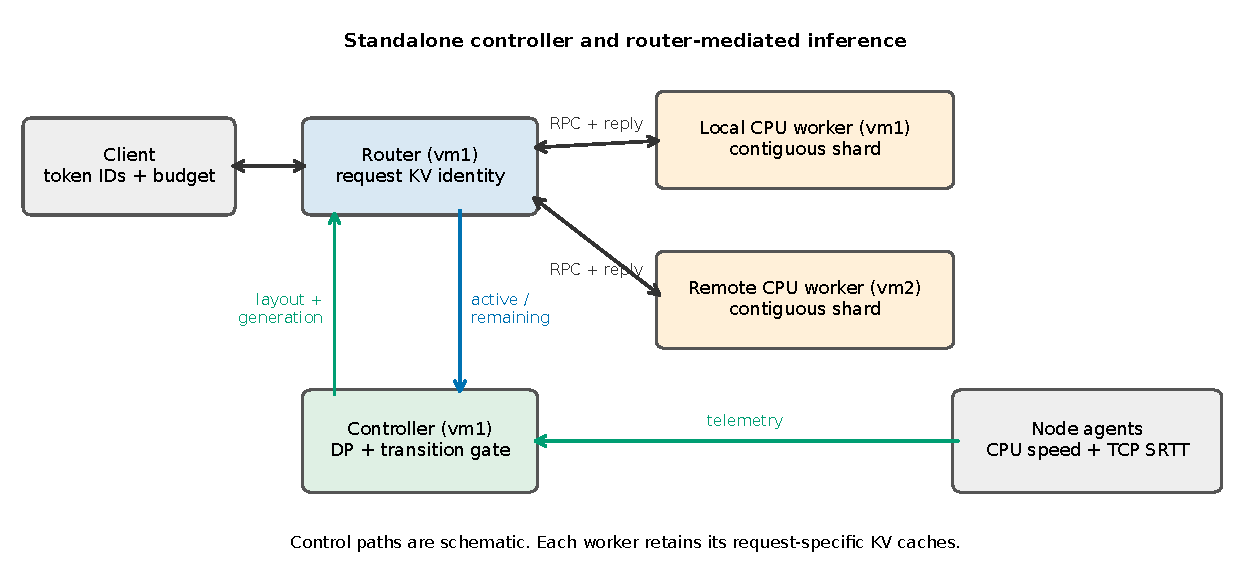
\includegraphics[width=1\textwidth,height=\textheight]{architecture.pdf}
\caption{Shardwise runtime. Inference follows router-issued worker
calls; control paths carry telemetry, layouts with generation numbers,
and request budgets. Host membership is shown in the labels.}
\end{figure}

\hypertarget{telemetry-and-control}{%
\subsection{Telemetry and control}\label{telemetry-and-control}}

Each machine runs a node agent that reports CPU speed relative to a
calibration profile and, where available, kernel TCP round-trip
estimates obtained with eBPF. Application-level call timings provide a
fallback for link costs. The router exports the number of active
requests, their remaining requested output tokens and an observation
timestamp. The controller rejects stale snapshots (older than 5 s, or
more than 2 s in the future), and holds voluntary movement when no
usable workload snapshot exists. Loss of a worker triggers recovery
placement immediately, bypassing voluntary gating.

\hypertarget{standalone-multi-device-deployment}{%
\subsection{Standalone, multi-device
deployment}\label{standalone-multi-device-deployment}}

Shardwise needs no Kubernetes installation; the controller discovers
workers from agent heartbeats. A packaged application (Section 7) adds
multi-device joining for any number of machines. One machine
\emph{invites}: it runs the controller and router and displays its
address and an eight-digit code. Every other machine \emph{joins} with
that code and runs one worker. Joining machines make only outbound
connections: each keeps a small pool of authenticated idle TCP
connections to the inviting machine, which splices one of them to a
local endpoint whenever its controller or router needs that worker. On a
joining machine the worker, node agent and dashboard listen only on the
loopback interface, so only the inviting machine must accept connections
from the network. This matters on campus networks and on Windows hosts,
whose firewalls block inbound traffic by default. Joining machines
receive controls (stop, restore, injected delay or slowdown) through a
one-second poll, and a machine that stops polling for 5 s is treated as
lost.

\hypertarget{decision-model}{%
\section{Decision model}\label{decision-model}}

\hypertarget{stage-cost-and-placement-objectives}{%
\subsection{Stage cost and placement
objectives}\label{stage-cost-and-placement-objectives}}

Let \(L\) denote decoder layers, \(W\) ordered workers, \(C\) context
length, and \(0=b_0\le b_1\le\cdots\le b_W=L\) layer boundaries. Worker
\(i\) (indexed from zero) receives \([b_i,b_{i+1})\). An empty interval
costs zero and is omitted at execution. For a nonempty interval
\([a,b)\) the controller uses

\[
d_i(a,b;C)=\frac{(b-a)c(C)+e\mathbf{1}_{a=0}+h\mathbf{1}_{b=L}}
 {\max(s_i,0.01)}+\ell_i. \tag{1}
\]

Here \(c(C)\) is per-layer compute time, \(e\) the embedding cost, \(h\)
the final normalisation and head cost, \(s_i\) relative compute speed,
and \(\ell_i\) the link cost into worker \(i\) (\(\ell_0=0\)). \(c(C)\)
is interpolated linearly between profiled contexts and clamped outside
them. Endpoint costs apply only to nonempty assignments. Equation (1)
does not model memory feasibility, transfer/compute overlap, or
prefill/decode interference.

For a placement \(\pi\), define the sequential cost
\(P(\pi)=\sum_i d_i\) and the bottleneck cost \(B(\pi)=\max_i d_i\). The
latency objective is \(J_{\rm lat}=P\) and the throughput objective
\(J_{\rm thr}=B\). Let \(F_o(w,j)\) be the best value of objective \(o\)
when the first \(j\) layers are assigned to the first \(w\) workers:

\[
F_o(w,j)=\min_{0\le a\le j}\phi_o\big(F_o(w-1,a),d_{w-1}(a,j;C)\big), \tag{2}
\]

with \(F_o(0,0)=0\), \(F_o(0,j>0)=+\infty\), \(\phi_{\rm lat}(x,y)=x+y\)
and \(\phi_{\rm thr}(x,y)=\max(x,y)\). The optimum is \(F_o(W,L)\);
stored predecessors recover the boundaries.

\textbf{Proposition 1 (exactness).} Equation (2) minimises the chosen
objective over all ordered contiguous assignments, including empty
workers, in \(O(WL^2)\) time and \(O(WL)\) space.

\emph{Proof.} Every feasible assignment of \(j\) layers to \(w\) workers
ends with a unique boundary \(a\), and its prefix is feasible for
\((w-1,a)\). Because addition and maximum are nondecreasing in the
prefix value, replacing the prefix by an optimal one cannot worsen the
total. Conversely every enumerated prefix and last interval is feasible.
Induction from the base state proves both directions. There are
\(O(WL)\) states with \(O(L)\) choices each. \(\square\)

An independent exhaustive checker confirms both objectives on 1,000
random small instances (2,000 checks), including empty assignments and
the speed floor.

\hypertarget{why-concurrency-changes-the-objective}{%
\subsection{Why concurrency changes the
objective}\label{why-concurrency-changes-the-objective}}

Consider an ideal stationary decode pipeline in which each active stage
is a single server with deterministic service time \(d_i\), and \(Q\)
closed-loop token streams must traverse all stages before emitting their
next token. Ignoring prefill, think time and transitions, the aggregate
token rate \(X_Q\) satisfies

\[X_Q\le\min\left(\frac{1}{B},\frac{Q}{P}\right),\qquad
 J_Q=\max\left(B,\frac{P}{Q}\right). \tag{3}\]

\textbf{Proposition 2 (capacity envelope).} Under these assumptions
Equation (3) bounds the stationary token rate.

\emph{Proof.} Every token needs \(d_i\) of service at stage \(i\), so
utilisation \(X_Qd_i\le1\) gives \(X_Q\le1/B\). A stream needs at least
\(P\) per cycle; Little's law for the closed network gives
\(Q=X_Q\bar r\) with mean cycle time \(\bar r\ge P\)
\citep{little1961proof}, so \(X_Q\le Q/P\). \(\square\)

Equation (3) is the familiar asymptotic bound of closed queueing
networks \citep{reiser1980mva}. Its consequence for placement is direct:
at \(Q=1\) the relevant cost is \(P\), so the sum objective is correct;
once \(Q\ge P/B\) it is \(B\). For two balanced stages, two concurrent
requests are enough for the bottleneck objective to matter. Shardwise's
automatic mode applies this rule, using the latency objective at
\(Q\le1\) and the throughput objective otherwise. Evaluated with profile
costs, (3) is an \emph{ideal envelope}, not a guarantee on measured
execution; Section 6.1 compares the two.

\hypertarget{transition-gate-finite-work-and-sensitivity}{%
\subsection{Transition gate, finite work, and
sensitivity}\label{transition-gate-finite-work-and-sensitivity}}

A voluntary candidate must first improve the objective by more than a
configured fraction (15\% here) after a cooldown (30 s). Recovery
placements bypass this check. The transition duration is estimated as

\[T=F+CpL, \tag{4}\]

where \(F\) prices fixed reconfiguration and \(p\) prices replay per
token-layer. The whole chain is priced because a generation change
rebuilds request state through every layer, including layers whose owner
does not change.

For current and candidate per-token costs \(j_c>j_n\) (seconds), horizon
\(H>0\) and margin \(m\ge0\), a move is admitted if

\[\frac{(H-T)_+}{j_n}>(1+m)\frac{H}{j_c}, \tag{5}\]

that is, if the tokens served in the remaining time after the transition
exceed those served without moving by the margin.

\textbf{Proposition 3 (payback boundary).} For \(T>0\), a finite horizon
satisfies (5) if and only if \(\Delta_m=j_c-(1+m)j_n>0\) and

\[H>H_m=\frac{Tj_c}{\Delta_m}. \tag{6}\]

\emph{Proof.} If \(H\le T\) the left side of (5) is zero. Otherwise
multiplying by the positive costs gives \(H\Delta_m>Tj_c\), which
requires \(\Delta_m>0\) and yields (6). Conversely (6) implies \(H>T\)
and reconstructs (5). \(\square\)

At \(m=0\) the boundary is \(Tj_c/(j_c-j_n)\), while a large margin can
make payback impossible however large the steady-state gain. The
optional remaining-work rule caps the horizon at \(H_R=\min(H,Rj_c)\),
where \(R\) is the sum of remaining requested output tokens over active
requests. By Proposition 3 it admits a move if and only if

\[\Delta_m>0,\quad H>H_m,\quad R>\frac{T}{\Delta_m}. \tag{7}\]

Condition (7) shows why small budgets suppress moves. It also reveals a
pitfall: \(R(t)\) is the work of the \emph{present} cohort. Each
generated token decreases it, but every newly admitted request adds a
full budget, so in a continuing service \(R(t)\) need not decrease.
Forecast errors enter the boundary through
\(\partial H_m/\partial T=j_c/\Delta_m\) and
\(\partial H_m/\partial j_n=Tj_c(1+m)/\Delta_m^2\); both grow as the
improvement approaches the margin, so marginal moves are the most
sensitive to an underestimated \(T\).

\hypertarget{methodology}{%
\section{Methodology}\label{methodology}}

\hypertarget{testbed-model-and-workloads}{%
\subsection{Testbed, model and
workloads}\label{testbed-model-and-workloads}}

The real-model evidence consists of three separately executed matrices
on two Azure virtual machines, each with two vCPUs and about 8 GiB of
RAM. Machine vm1 hosts the controller, router and one worker; vm2 hosts
the second worker. The model is Qwen3-0.6B \citep{yang2025qwen3} (28
decoder layers), executed on CPU in FP32 with KV caching and one thread
per worker, using PyTorch 2.14 and Transformers 5.17
\citep{paszke2019pytorch, wolf2020transformers}. Clients run a closed
loop with concurrency \(Q\in\{1,2\}\) and 64-token prompts.

\begin{itemize}
\tightlist
\item
  \textbf{Adaptation matrix (30 runs).} A 120 ms network delay and a
  0.5-CPU cgroup quota on the remote worker, each under static,
  hysteresis, gate and forced-gate policies with three repeats; and
  worker loss under static, hysteresis and gate with two repeats. Phases
  are 40 s before, 120 s during and 60 s after the fault; 64 output
  tokens. Three single-device runs provide a same-runtime baseline.
\item
  \textbf{Objective matrix (20 runs).} Latency and throughput objectives
  at \(Q=1,2\), three repeats under stable conditions and two under a
  120 ms delay; 32 output tokens; 10/40/10 s phases.
\item
  \textbf{Demand matrix (12 runs).} Fixed throughput, automatic
  objective with a fixed 30 s horizon, and automatic objective with a
  remaining-work horizon, at \(Q=1,2\) with two repeats; 64 output
  tokens.
\end{itemize}

The profile used by the controller has per-layer costs of 6.567, 7.662,
9.071 and 12.681 ms at contexts 128, 512, 1024 and 2048, embedding 0.071
ms, head 50.49 ms, fixed transition 1,740 ms and replay 0.3667 ms per
token-layer; at context 128 the forecast transition is 3,054 ms. The
gate uses a 30 s horizon and 13\% margin. Seeds for all schedules are
recorded. Six pilot or interrupted runs are archived separately and
excluded from the 65 completed runs.

\hypertarget{metrics}{%
\subsection{Metrics}\label{metrics}}

Whole-run throughput is successful output tokens divided by the time
from the measurement start to the later of the nominal end and the last
completion; drain and transitions are therefore included. Fault-phase
throughput counts the tokens of requests completing between the logged
fault boundaries. Because tokens are attributed at completion, phase
metrics move in steps of whole requests; we always report them next to
whole-run metrics. Client latency uses external start and completion
timestamps. Failed requests remain in all denominators.

\hypertarget{analysis}{%
\subsection{Analysis}\label{analysis}}

Runs are the unit of analysis. We report medians across repeats and show
every run in the figures. Comparisons are stated either as ratios of
medians or as repeat-matched relative differences and are labelled as
such. With two or three repeats per condition we make no significance
claims; effects are descriptive. An independent analysis recomputes all
65 runs and 939 requests from raw logs and verifies source and data
hashes.

\hypertarget{supporting-evidence-strata}{%
\subsection{Supporting evidence
strata}\label{supporting-evidence-strata}}

Four further studies diagnose mechanisms and are never pooled with the
real-model runs: (i) a deterministic cost-model ablation of 240
placements and 18,000 gate evaluations; (ii) a synthetic loopback study
of 78 windows and 85,116 calls that decomposes communication residuals;
(iii) a replay of 71 recorded voluntary candidates under ten policies;
and (iv) synthetic routing probes. We label each result with its
stratum.

\hypertarget{results}{%
\section{Results}\label{results}}

\hypertarget{rq1-concurrency-decides-the-objective}{%
\subsection{RQ1: concurrency decides the
objective}\label{rq1-concurrency-decides-the-objective}}

Table 2 and Figure 2 summarise the objective matrix. Under stable
conditions with two concurrent requests, throughput placement splits the
model into a pipeline and achieves a median 7.303 tokens/s, against
4.046 for latency placement, which keeps all layers on one machine: an
80.5\% increase. The gain is not bought at the expense of individual
users: median completion time falls from 15.777 to 8.739 s for 32-token
answers. With one request, the two objectives are close (4.029 vs 3.875
tokens/s), as the envelope predicts: with no second request, there is
nothing to overlap with the added stage.

The network perturbation separates them. With one request and a 120 ms
delay, latency placement retains 4.001 tokens/s and throughput placement
drops to 2.419, a 65.4\% advantage for latency placement; median
completion is 8.012 versus 12.531 s. With two requests, throughput
placement still wins (4.778 vs 4.040 tokens/s) but by a smaller margin.
Figure 3 shows that the ideal envelope (3) captures the direction of
these effects: the profile predicts a large gain from the pipeline at
\(Q=2\) and none at \(Q=1\).

\begin{figure}
\centering
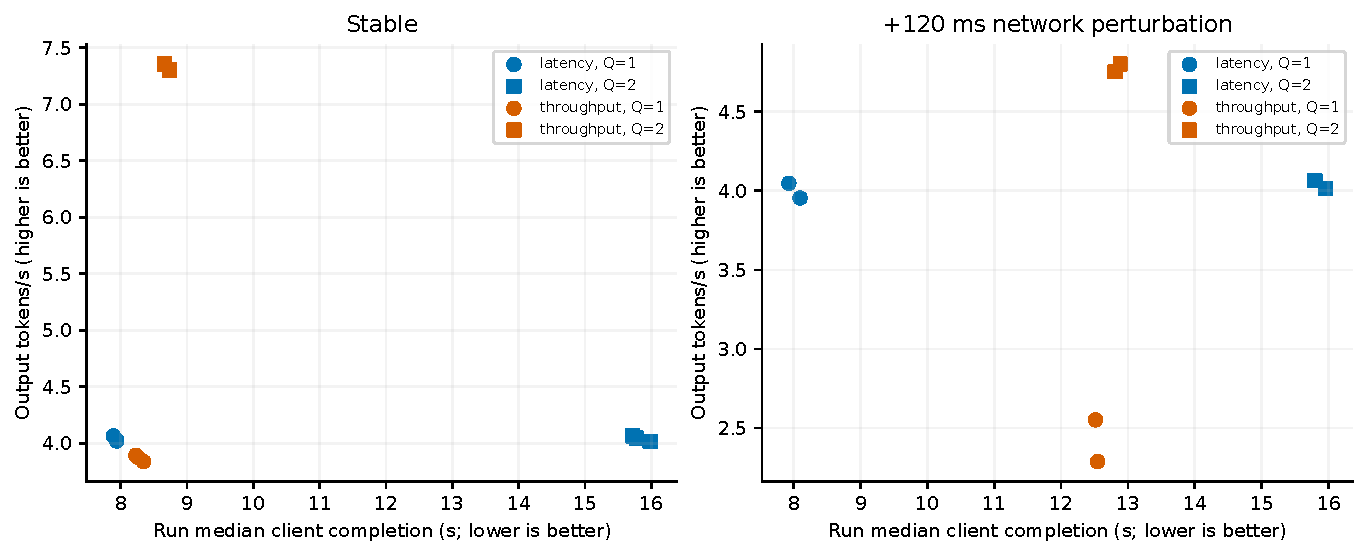
\includegraphics[width=1\textwidth,height=\textheight]{objective-frontier.pdf}
\caption{Objective trade-off frontier. Each marker is one real-model
run; circles denote one concurrent request and squares two. Completion
time and whole-run throughput include transitions and drain.}
\end{figure}

\begin{figure}
\centering
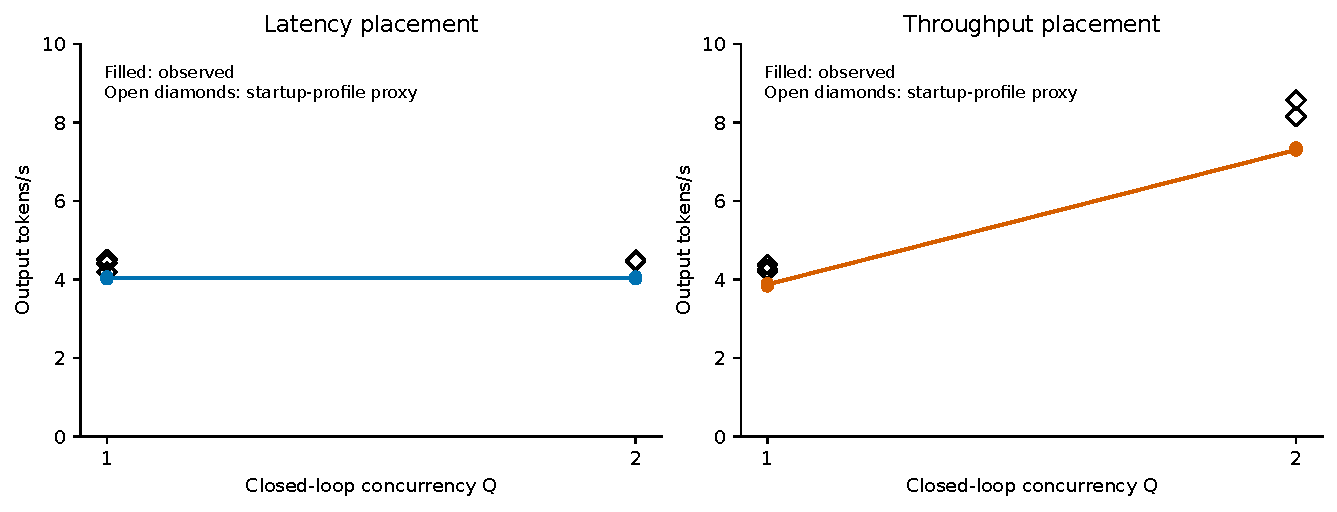
\includegraphics[width=1\textwidth,height=\textheight]{service-envelope.pdf}
\caption{Ideal profile envelope from Equation (3) (open diamonds) and
measured stable-run throughput (filled points). The envelope ignores
prefill, transitions and runtime overhead.}
\end{figure}

\begin{table}[htbp]
\centering\small
\caption{Whole-run objective and demand results. Q denotes closed-loop concurrency; N is requested output tokens. Medians use runs as units; drain is included.}
\begin{tabular}{lllrrrr}
\toprule
Matrix & Condition & Arm & Q & N & Runs & Tokens/s \\
\midrule
demand & stable & auto-fixed & 1 & 64 & 2 & 4.207 \\
demand & stable & auto-remaining & 1 & 64 & 2 & 4.107 \\
demand & stable & throughput & 1 & 64 & 2 & 4.054 \\
demand & stable & auto-fixed & 2 & 64 & 2 & 5.944 \\
demand & stable & auto-remaining & 2 & 64 & 2 & 5.729 \\
demand & stable & throughput & 2 & 64 & 2 & 7.830 \\
objective & network & latency & 1 & 32 & 2 & 4.001 \\
objective & network & throughput & 1 & 32 & 2 & 2.419 \\
objective & network & latency & 2 & 32 & 2 & 4.040 \\
objective & network & throughput & 2 & 32 & 2 & 4.778 \\
objective & stable & latency & 1 & 32 & 3 & 4.029 \\
objective & stable & throughput & 1 & 32 & 3 & 3.875 \\
objective & stable & latency & 2 & 32 & 3 & 4.046 \\
objective & stable & throughput & 2 & 32 & 3 & 7.303 \\
\bottomrule
\end{tabular}
\end{table}


\textbf{Answer to RQ1.} The useful objective depends on concurrency and
network conditions. For one interactive user, keeping the model on one
machine is the safe default; for two or more overlapping requests the
bottleneck objective gives a large gain in both throughput and
completion time.

\hypertarget{rq2-adaptation-pays-a-transition-cost}{%
\subsection{RQ2: adaptation pays a transition
cost}\label{rq2-adaptation-pays-a-transition-cost}}

\textbf{Starting in the wrong layout is expensive.} In the demand
matrix, automatic policies start in the latency layout and must observe
two concurrent requests before moving to the pipeline. Fixed throughput
placement achieves 7.830 tokens/s; automatic placement with the fixed
horizon achieves 5.944 (24.1\% lower) and with the remaining-work
horizon 5.729. The moves occur 30.0 s after initial assignment, exactly
when the cooldown expires. Most of the gap is therefore the time spent
in the wrong layout plus the transition itself.

\textbf{Phase gains overstate whole-run gains.} Table 3 and Figure 4
report the adaptation matrix. Under the CPU quota, static placement
keeps the slowed worker's share and falls to 4.215 tokens/s during the
fault, while adaptive policies re-balance and reach about 5.27: a 25.0\%
ratio-of-medians gain (25.3\% repeat-matched). Over the whole run,
including pre- and post-fault phases and drain, the gain shrinks to
6.8\% for hysteresis (6.133 vs 5.744) and 5.2\% for the gate. Under the
network delay, fault-phase throughput is the same for all policies
(about 5.27), but over the whole run the adaptive policies are 6.4-7.6\%
\emph{slower} than static (6.131 and 6.055 vs 6.554 tokens/s): their
moves cost more than they returned within the window.

\textbf{Recovery is where adaptation is indispensable.} When a worker is
lost, static placement completes no request during the fault and records
19 failures across its two runs. Hysteresis and the gate re-place the
model on the surviving machine, record no failures, and sustain 4.219
and 3.693 tokens/s during the fault. The same-runtime single-device
baseline reaches 4.158 tokens/s at \(Q=2\); it shares the runtime and
therefore isolates distribution effects rather than comparing against an
optimised engine.

\begin{table}[htbp]
\centering\small
\caption{Adaptation and separate baseline results. Phase throughput attributes tokens at completion between logged on/off times. Whole-run throughput includes drain. Failures are retained.}
\begin{tabular}{llrrrr}
\toprule
Condition & Arm & Runs & Phase TPS & Whole TPS & Failures \\
\midrule
single-device & static & 3 & 4.267 & 4.158 & 0 \\
compute & gate & 3 & 5.267 & 6.041 & 0 \\
compute & gate-force & 3 & 5.268 & 6.100 & 0 \\
compute & hysteresis & 3 & 5.269 & 6.133 & 0 \\
compute & static & 3 & 4.215 & 5.744 & 0 \\
loss & gate & 2 & 3.693 & 5.409 & 0 \\
loss & hysteresis & 2 & 4.219 & 5.443 & 0 \\
loss & static & 2 & 0.000 & 3.271 & 19 \\
network & gate & 3 & 5.270 & 6.055 & 0 \\
network & gate-force & 3 & 5.271 & 6.117 & 0 \\
network & hysteresis & 3 & 5.269 & 6.131 & 0 \\
network & static & 3 & 5.270 & 6.554 & 0 \\
\bottomrule
\end{tabular}
\end{table}


\begin{figure}
\centering
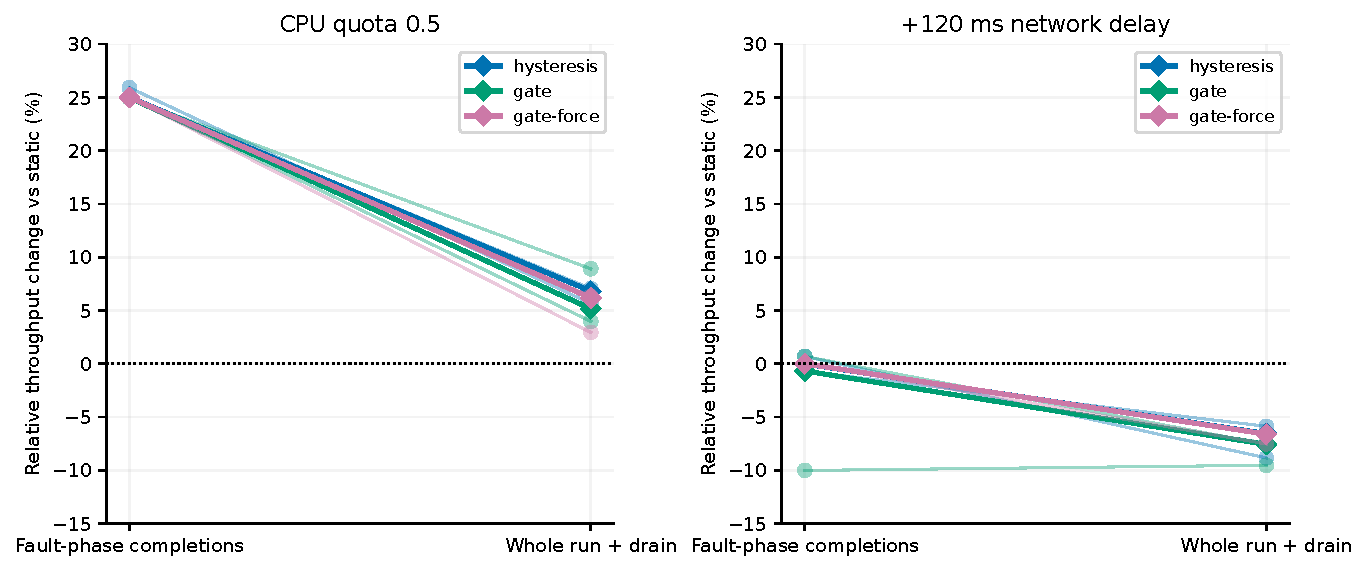
\includegraphics[width=1\textwidth,height=\textheight]{adaptation-comparison.pdf}
\caption{Repeat-matched adaptation contrasts against static placement.
Thin paths show individual repeat blocks and thick paths their median.
Moving from fault-phase to whole-run throughput reveals transition,
post-fault and drain costs.}
\end{figure}

\begin{figure}
\centering
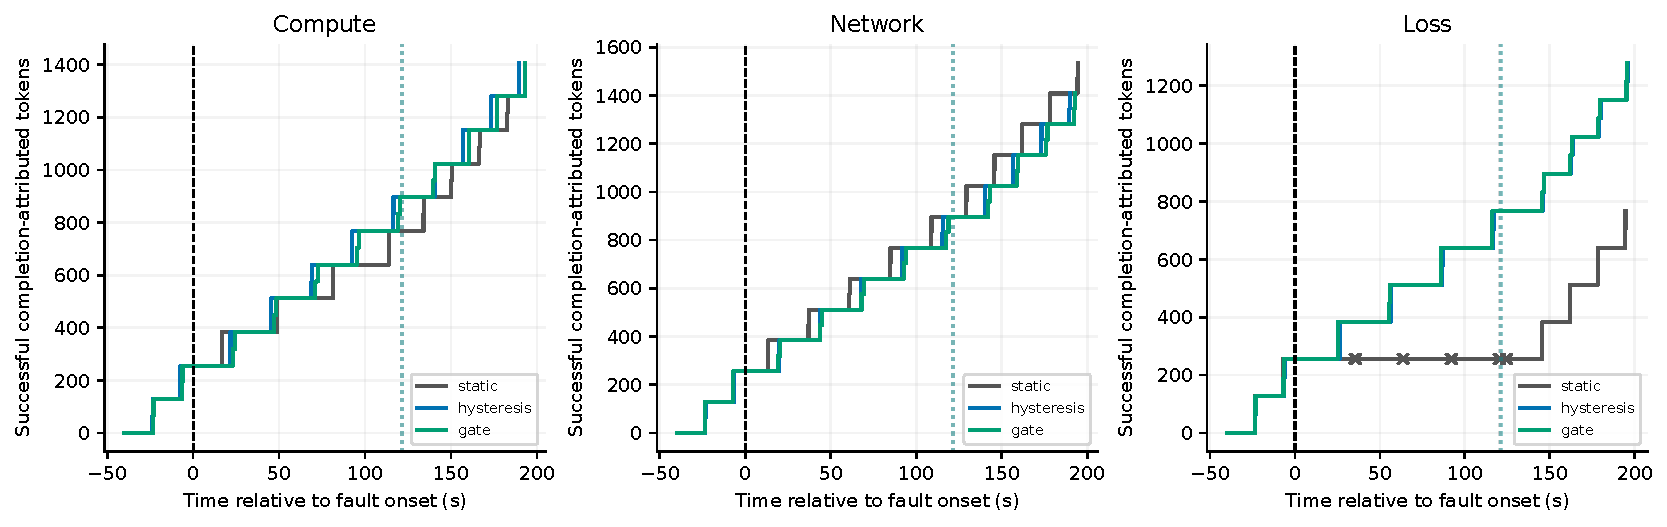
\includegraphics[width=1\textwidth,height=\textheight]{fault-traces.pdf}
\caption{Completion traces for compute degradation, network delay and
worker loss. For each policy the run closest to the policy median is
shown. Vertical markers are fault boundaries; crosses are failed
requests; tokens are attributed at completion.}
\end{figure}

\textbf{Answer to RQ2.} Adaptation repays its cost under availability
loss and, to a lesser degree, under sustained compute degradation, but
not under a moderate network delay in a few-minute window. Reporting
only fault-phase throughput would have overstated the compute benefit by
a factor of 3.7 and hidden the network loss.

\hypertarget{rq3-budget-horizons-and-renewing-work}{%
\subsection{RQ3: budget horizons and renewing
work}\label{rq3-budget-horizons-and-renewing-work}}

Figure 5 follows both two-request demand runs. In the remaining-work
run, four eligible candidates at about 23, 25, 27 and 29 s are rejected
while the recorded budget falls through 32, 23, 14 and 5 tokens; each
rejection matches condition (7). New closed-loop admissions then raise
the budget to 127 tokens and the move executes at 31.0 s. In the other
repeat the move executes at 23.0 s with 33 remaining tokens. The rule
therefore behaves exactly as designed, but in a continuing service the
cohort it budgets is replaced before the decision matters, and the
result is a delayed move rather than an avoided one. With one request,
automatic and fixed policies are within 4\% of each other (4.207 vs
4.054 tokens/s).

\begin{figure}
\centering
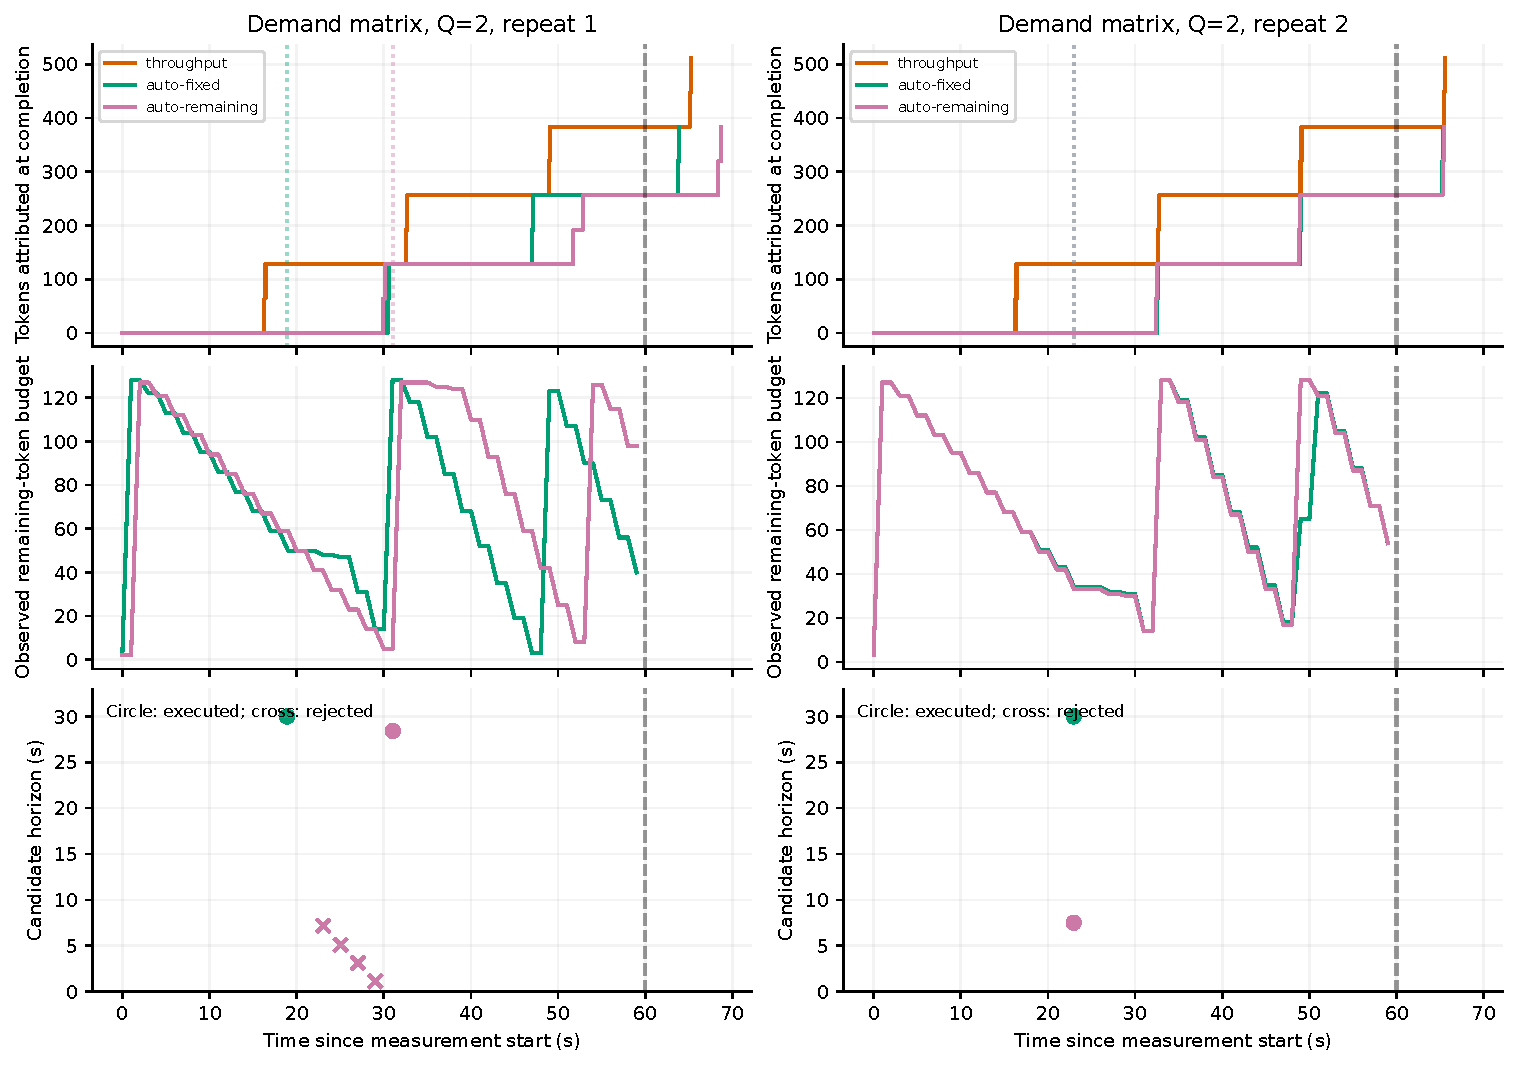
\includegraphics[width=1\textwidth,height=\textheight]{demand-timeline.pdf}
\caption{Both two-request demand repeats. Top: cumulative tokens
credited at completion. Middle: remaining active-token budget, which
rises after new admissions. Bottom: planning horizons and voluntary
candidates; circles execute and crosses reject. The 60 s line marks the
end of admission.}
\end{figure}

\textbf{Answer to RQ3.} A present-work budget correctly blocks moves
that cannot pay back within the current cohort, but it is the wrong
quantity for a service with continuing arrivals. Horizon semantics must
match the workload: the remaining work of a finite cohort, or a forecast
of future demand for a continuing one.

\hypertarget{rq4-diagnostics-that-can-reverse-conclusions}{%
\subsection{RQ4: diagnostics that can reverse
conclusions}\label{rq4-diagnostics-that-can-reverse-conclusions}}

\textbf{Transitions are underpriced.} Grouping disrupted requests by
executed decision yields 34 transitions: 16 under compute faults with
mean 5,382 ms (SD 1,839) and 18 under network faults with mean 3,948 ms
(SD 598), against a forecast of 3,054 ms (Figure 6). The forecast is low
by 76.2\% and 29.2\%. Since \(H_m\) in (6) is proportional to \(T\), the
payback horizon is underestimated by the same factors, and moves that
pass the gate can fail to repay, which is consistent with the network
result in Section 6.2.

\begin{figure}
\centering
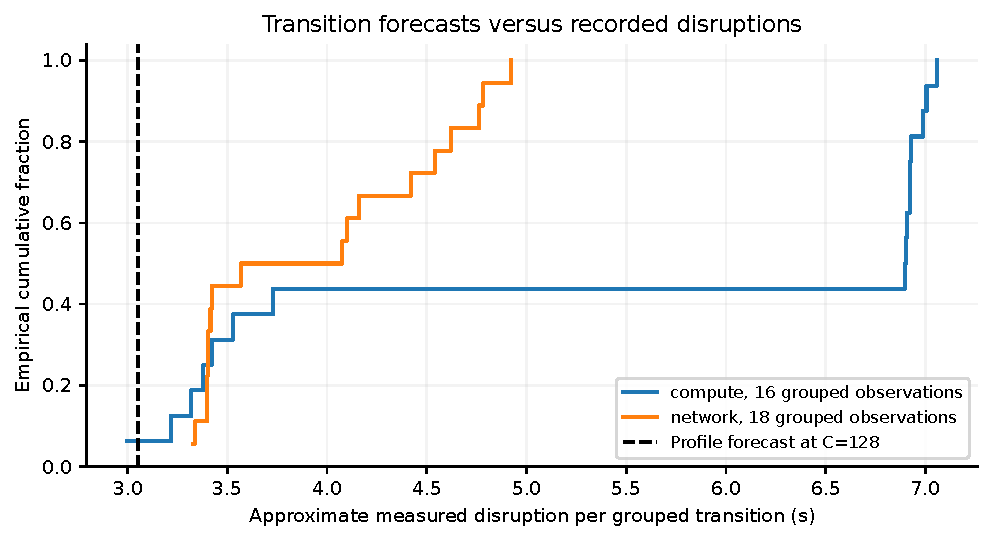
\includegraphics[width=1\textwidth,height=\textheight]{transition-forecast.pdf}
\caption{Distribution of 34 grouped transition durations; the dashed
line is the profile forecast.}
\end{figure}

\textbf{Application timings measure queues, not links.} In a synthetic
loopback study (no model, no physical network) with 50 ms service and
four concurrent callers, the mean call-minus-compute residual is 149.98
ms, of which 148.80 ms is time spent waiting for the worker. Subtracting
the measured wait leaves 1.18 ms: 99.2\% of what an application-level
estimator would call link cost is queueing (Figure 7). Admission control
at the client removes the contamination from the estimate but not from
the user's experience: mean completion is 204.5 ms with admission versus
200.1 ms without. A controller that prices links from application
timings will therefore see congestion as network cost and may move
layers for the wrong reason.

\begin{figure}
\centering
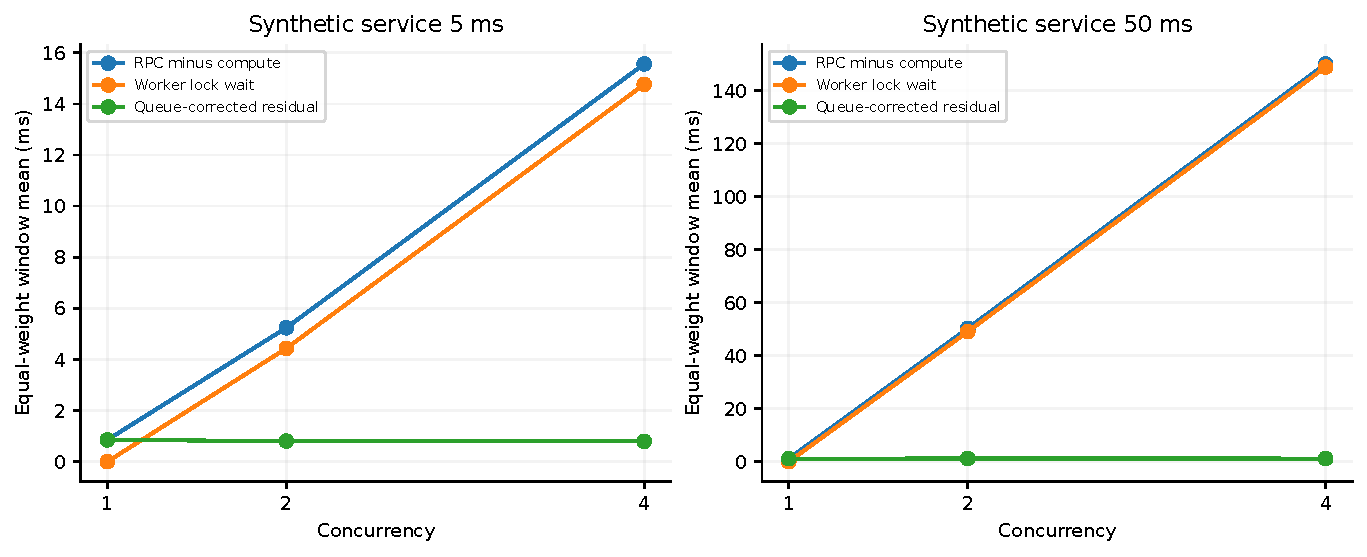
\includegraphics[width=1\textwidth,height=\textheight]{queue-decomposition.pdf}
\caption{Synthetic decomposition of call-minus-compute residuals for 5
ms and 50 ms service. Residuals grow with concurrency, while subtracting
measured worker wait leaves a small remainder. Each point is one
window.}
\end{figure}

\textbf{Omitted cost terms change the chosen split.} In the
deterministic ablation, at context 2048 with equal speeds and a 0.5 ms
hop, the full model selects a 16/12 split with bottleneck 158.18 ms.
Omitting the embedding and head costs selects 14/14 and scores 177.16 ms
(12.0\% worse); freezing the per-layer cost at its context-128 value
selects 18/10 and scores 170.91 ms (8.0\% worse). In the corresponding
gate sweep, a candidate improving the bottleneck from 225.8 to 185.1 ms
needs 77.9 s to repay a full-chain transition at zero margin and 190.9 s
at 13\%; it would be rejected by a 30 s horizon despite an 18\%
steady-state gain (Figure 8).

\begin{figure}
\centering
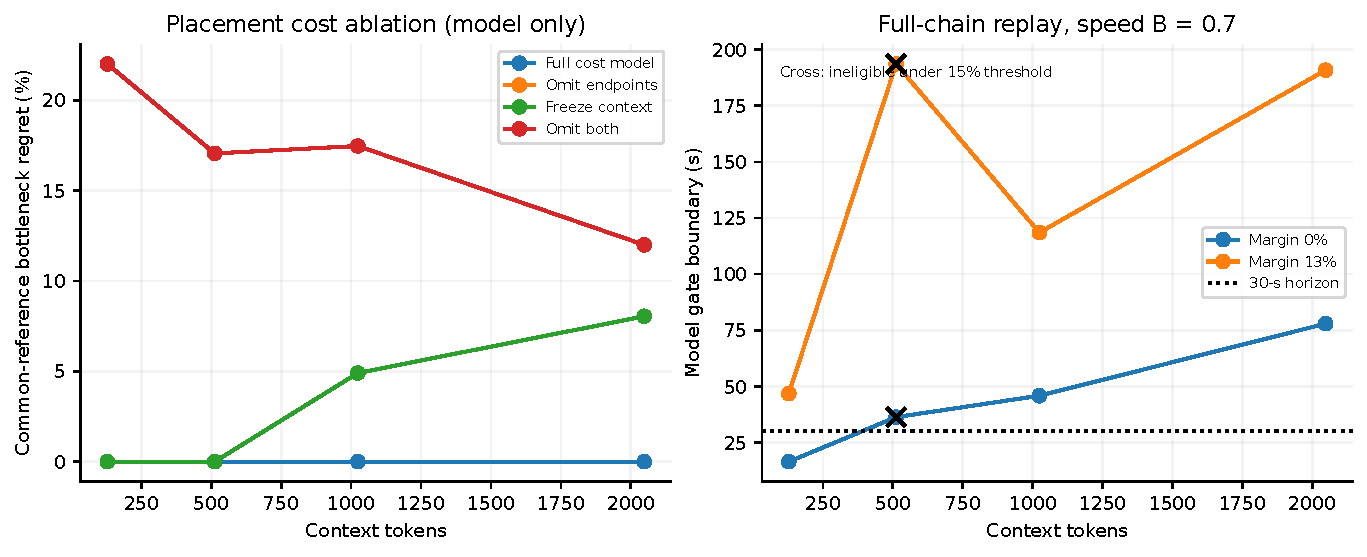
\includegraphics[width=1\textwidth,height=\textheight]{cost-and-gate-sensitivity.pdf}
\caption{Cost-model sensitivity. Left: bottleneck regret when cost terms
are omitted, rescored with the full model. Right: payback horizons for
selected transitions; crosses fail the separate improvement threshold.
Deterministic model outputs.}
\end{figure}

\textbf{Policy replay.} Replaying the 71 recorded voluntary candidates,
the fixed 30 s/13\% gate accepts 28; remaining budgets of 16 and 64
tokens accept none, while 256 and 1,024 accept 28; online calibration of
\(T\) accepts 19; and oracles with knowledge of phase boundaries or
future telemetry accept 51 and 32. Calibrating the transition forecast
alone thus removes a third of the accepted moves.

\textbf{Baselines can reverse the comparison.} In synthetic routing
probes with sleep-based workers, a three-stage pipeline (19.85 tokens/s)
beats replicas dispatched cyclically (14.99), but replicas dispatched to
the first available worker with FIFO admission reach 20.25 and overtake
it (Figure 9). A distributed pipeline must therefore be compared against
a well-dispatched replica baseline, not a naive one.

\begin{figure}
\centering
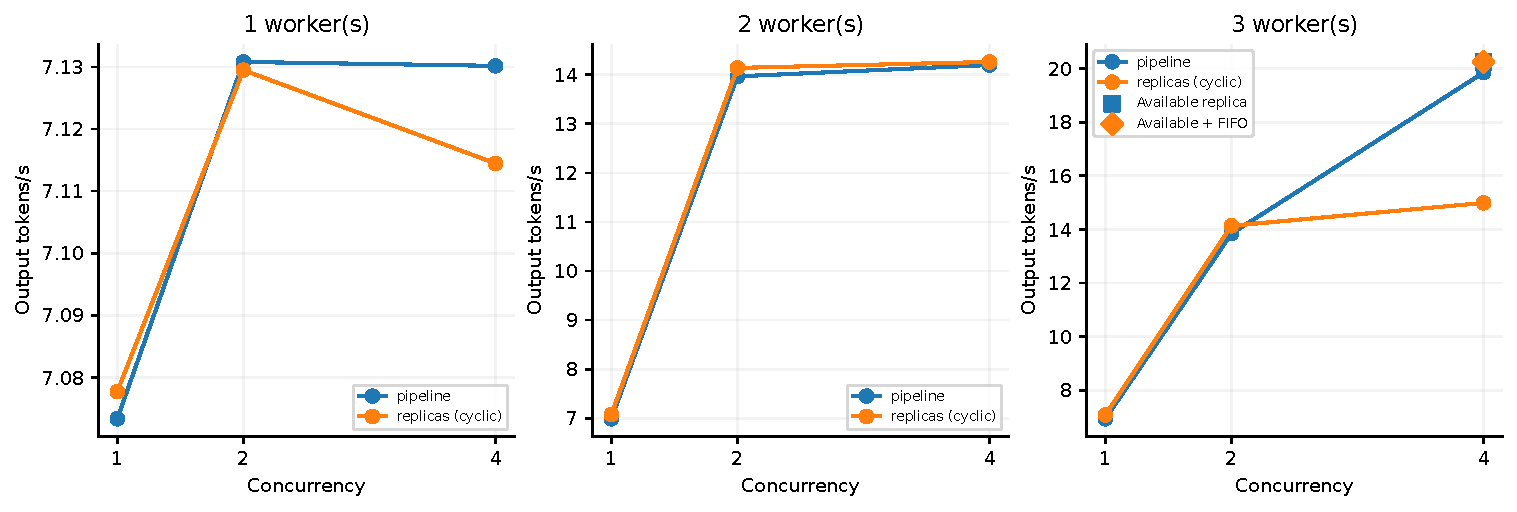
\includegraphics[width=1\textwidth,height=\textheight]{routing-sensitivity.pdf}
\caption{Synthetic routing sensitivity across worker counts and
concurrency. Cyclic replicas and pipeline stages are compared with
available-replica dispatch with and without FIFO admission. Sleep-based
workers on one host.}
\end{figure}

\textbf{Answer to RQ4.} Transition underpricing, queue-contaminated link
estimates, omitted endpoint and context terms, and weak baselines each
change which policy appears better. All four must be controlled before
an adaptive placement result can be trusted.

\hypertarget{deployment-and-correctness-validation}{%
\section{Deployment and correctness
validation}\label{deployment-and-correctness-validation}}

We packaged Shardwise as an installable application for Ubuntu (natively
or under Windows WSL2), with CPU and NVIDIA back-ends selected
automatically, a browser dashboard that shows only measured values, and
the multi-device joining of Section 3.4. The Debian package (about 48
MB, model downloaded on first run) is built and install-tested on clean
Ubuntu 22.04 and 24.04 images by continuous integration on every change.

\textbf{Multi-device function.} We validated joining, splitting and
recovery with three nodes, each a container with its own network
namespace and address, running the packaged application. This testbed
shares one 4-vCPU host, so it validates behaviour, not performance. With
Qwen3-0.6B, three nodes split the model into 12, 11 and 5 layers within
seconds of joining. Every transition below was timed by the application
from the triggering event to the first complete, contiguous, live
pipeline, in two complete scenario executions: stopping a joined worker
7.8 and 6.9 s; restoring it 11.3 and 9.1 s; a joined machine leaving
gracefully 8.1 and 6.2 s; and a joined machine killed without notice 5.4
and 5.4 s, measured from its last contact. Requests issued while a
worker was being stopped completed successfully, as did requests served
by the remaining machines after each loss. A wrong pairing code was
rejected before any model download, and a machine that rejoined was
re-admitted and re-placed.

\textbf{Numerical fidelity.} Splitting must not change model output. In
the demand matrix, all 12 runs pass a fixed-input greedy check against
an unsplit reference. For the application's default model,
Qwen2.5-0.5B-Instruct \citep{qwen2025qwen25}, a two-stage split produces
token sequences identical to unsplit Hugging Face greedy decoding for
both tested prompts (48 output tokens each), with the reference's
repetition penalty disabled to match greedy semantics.

\hypertarget{discussion}{%
\section{Discussion}\label{discussion}}

\hypertarget{guidelines-for-deployers}{%
\subsection{Guidelines for deployers}\label{guidelines-for-deployers}}

The results suggest five practical guidelines for small distributed
deployments.

\begin{enumerate}
\def\labelenumi{\arabic{enumi}.}
\tightlist
\item
  \textbf{Choose the objective from expected concurrency, before
  serving.} Use sum (latency) placement, usually a single machine, for
  one interactive user without speculative decoding, and bottleneck
  placement when two or more requests overlap. Starting in the right
  layout avoided a 24\% whole-run loss caused by waiting to discover it.
\item
  \textbf{Adapt for availability first.} Re-placement on device loss
  turned 19 failures into none; voluntary re-balancing returned 5-7\% at
  best in a few-minute window and lost 6-8\% under a moderate network
  delay.
\item
  \textbf{Calibrate transition cost online.} Profile-based forecasts
  were 29-76\% low. A payback gate is only as good as \(T\), and is most
  sensitive exactly for marginal moves.
\item
  \textbf{Do not price links from application timings without
  subtracting queueing.} Most of what such timings attribute to the
  network can be waiting.
\item
  \textbf{Match the horizon to the workload and the baseline to the
  claim.} A present-cohort budget suits finite batches, not continuing
  services; and a pipeline should beat a well-dispatched replica
  baseline, not a naive one.
\end{enumerate}

\hypertarget{threats-to-validity}{%
\subsection{Threats to validity}\label{threats-to-validity}}

\emph{Internal validity.} With two or three repeats per condition,
effects are descriptive; small differences (for example the 4\%
difference at \(Q=1\) in the demand matrix) are within run-to-run
variation. Phase metrics attribute tokens at completion and can leak
across boundaries, which is why whole-run metrics are reported
alongside. The three matrices use different source snapshots, which are
archived, and are never pooled. Transition durations are grouped from
request disruptions because explicit transition identifiers were not
logged.

\emph{Construct validity.} Fixed output budgets stand in for chat turns,
and closed-loop clients stand in for users; we do not measure answer
quality or user satisfaction. Router time-to-first-token is internal,
not streamed to the client.

\emph{External validity.} Two similar cloud VMs and one 0.6B CPU model
do not represent a heterogeneous consumer network, GPUs, or models that
exceed one machine's memory; there, capacity aggregation rather than
placement choice becomes the dominant motive, as in prior systems
\citep{tpi2025, prima2026}. The multi-device validation shares one
physical host, and the outbound-only joining property was verified from
the code and from that testbed, not with a deny-inbound firewall on
physical machines. The same-runtime single-device baseline isolates
distribution effects but is not an optimised inference engine such as
llama.cpp \citep{gerganov2023llamacpp}, and no prior system was
reproduced on our testbed.

\emph{Conclusion validity.} Synthetic, analytical and replay studies
establish mechanisms and sensitivities, not hardware outcomes; replayed
decisions cannot reveal the outcomes of moves that were not executed.

\hypertarget{future-work}{%
\subsection{Future work}\label{future-work}}

The most informative next experiments are a matched-start finite-cohort
study that varies only the horizon rule, transition measurements with
explicit identifiers across contexts and split distances, comparisons
against optimised single-device and replica baselines, and evaluation on
physically distinct consumer machines and models that do not fit on one
of them.

\hypertarget{conclusion}{%
\section{Conclusion}\label{conclusion}}

Splitting a small language model across commodity machines pays off
under two conditions: requests must overlap, so that pipeline stages
have parallel work, or a machine must fail, so that adaptation preserves
availability. Outside these conditions, distribution and voluntary
re-partitioning can cost more than they return. Using Shardwise and 65
audited real-model runs, we quantified both sides: an 80.5\% gain from
the right objective at two concurrent requests, a 65.4\% loss from the
wrong one for a single delayed request, a fault-phase gain of 25\% that
shrinks to 7\% over the whole run, and zero failures instead of 19 under
device loss. Our decision model explains these outcomes, and our
diagnostics show how transition underpricing, queue-contaminated
telemetry, renewing workloads and weak baselines can distort them. We
release the runtime, the installable multi-device application and every
raw trace so that these results can be checked and extended.

\hypertarget{data-and-code-availability}{%
\section{Data and code availability}\label{data-and-code-availability}}

The repository contains the runtime, the packaged application, raw
request, telemetry, event and decision logs, archived source snapshots
for every matrix, hash manifests, and the analysis scripts that
regenerate every table and figure
(\texttt{docs/paper/elsevier/analyze.py}, \texttt{figures.py}). The
dataset registry is \texttt{results/experiments.json}. Raw artifacts
predate the project's renaming and use its former name, KubeEdgeInfer;
machine labels vm1/vm2 in this paper correspond to vm2/vm3 in the raw
logs. A public repository URL and archival DOI will be provided on
acceptance.

\hypertarget{credit-authorship-contribution-statement}{%
\section{CRediT authorship contribution
statement}\label{credit-authorship-contribution-statement}}

To be completed by the authors.

\hypertarget{declaration-of-competing-interest}{%
\section{Declaration of competing
interest}\label{declaration-of-competing-interest}}

To be completed by the authors.

\hypertarget{declaration-of-generative-ai-and-ai-assisted-technologies-in-the-manuscript-preparation-process}{%
\section{Declaration of generative AI and AI-assisted technologies in
the manuscript preparation
process}\label{declaration-of-generative-ai-and-ai-assisted-technologies-in-the-manuscript-preparation-process}}

During the preparation of this work the authors used AI coding and
writing assistants (OpenAI Codex and Anthropic Claude) for literature
discovery, analysis-script preparation, artifact auditing, software
development and drafting. After using these tools, the authors reviewed
and edited the content as needed and take full responsibility for the
content of the published article. \emph{(Authors: confirm or revise this
statement after your review.)}

\bibliographystyle{elsarticle-num}
\bibliography{references}
\end{document}
